%%%%%%%%%%%%%%%%%%%%%%%%%%%%%%%%%%%%%%%%%%%%%%%%%%%%%%%%%%%%
% File: hw.tex 						   %
% Description: LaTeX template for homework.                %
%
% Feel free to modify it (mainly the 'preamble' file).     %
% Contact hfwei@nju.edu.cn (Hengfeng Wei) for suggestions. %
%%%%%%%%%%%%%%%%%%%%%%%%%%%%%%%%%%%%%%%%%%%%%%%%%%%%%%%%%%%%

%%%%%%%%%%%%%%%%%%%%%%%%%%%%%%%%%%%%%%%%%%%%%%%%%%%%%%%%%%%%%%%%%%%%%%
% IMPORTANT NOTE: Compile this file using 'XeLaTeX' (not 'PDFLaTeX') %
%
% If you are using TeXLive 2016 on windows,                          %
% you may need to check the following post:                          %
% https://tex.stackexchange.com/q/325278/23098                       %
%%%%%%%%%%%%%%%%%%%%%%%%%%%%%%%%%%%%%%%%%%%%%%%%%%%%%%%%%%%%%%%%%%%%%%

\documentclass[11pt, a4paper, UTF8]{ctexart}
%%%%%%%%%%%%%%%%%%%%%%%%%%%%%%%%%%%
% File: preamble.tex
%%%%%%%%%%%%%%%%%%%%%%%%%%%%%%%%%%%

\usepackage[top = 1.5cm]{geometry}

% Set fonts commands
\newcommand{\song}{\CJKfamily{song}} 
\newcommand{\hei}{\CJKfamily{hei}} 
\newcommand{\kai}{\CJKfamily{kai}} 
\newcommand{\fs}{\CJKfamily{fs}}

\newcommand{\me}[3]{\author{{\bfseries 姓名:}\underline{#1}\hspace{2em}{\bfseries 学号:}\underline{#2}\hspace{2em}{\bfseries 邮箱:}\underline{#3}}}

% Always keep this.
\newcommand{\noplagiarism}{
  \begin{center}
    \fbox{\begin{tabular}{@{}c@{}}
      请独立完成作业,不得抄袭。\\
      若参考了其它资料,请给出引用。\\
      鼓励讨论,但需独立书写解题过程。
    \end{tabular}}
  \end{center}
}

% Each hw consists of three parts:
% (1) this homework
\newcommand{\beginthishw}{\part{作业}}
% (2) corrections (Optional)
\newcommand{\begincorrection}{\part{订正}}
% (3) any feedback (Optional)
\newcommand{\beginfb}{\part{反馈}}

% For math
\usepackage{amsmath}
\usepackage{amsfonts}
\usepackage{amssymb}

% Define theorem-like environments
\usepackage[amsmath, thmmarks]{ntheorem}

\theoremstyle{break}
\theorembodyfont{\song}
\theoremseparator{}
\newtheorem*{problem}{Problem}





\theorempreskip{2.0\topsep}
\theoremheaderfont{\kai\bfseries}
\theoremseparator{:}
% \newtheorem*{remark}{注}
\theorempostwork{\bigskip\hrule}
\newtheorem*{solution}{Solution}
\theorempostwork{\bigskip\hrule}
\newtheorem*{reference}{Reference}

\theoremstyle{plain}
\newtheorem*{cause}{错因分析}
\newtheorem*{remark}{注}

\theoremstyle{break}
\theorempostwork{\bigskip\hrule}
\theoremsymbol{\ensuremath{\Box}}
\newtheorem*{proof}{Proof}

\renewcommand\figurename{图}
\renewcommand\tablename{表}

% For figures
% for fig with caption: #1: width/size; #2: fig file; #3: fig caption
\newcommand{\fig}[3]{
  \begin{figure}[htp]
    \centering
      \includegraphics[#1]{#2}
      \caption{#3}
  \end{figure}
}

% for fig without caption: #1: width/size; #2: fig file
\newcommand{\fignocaption}[2]{
  \begin{figure}[htp]
    \centering
    \includegraphics[#1]{#2}
  \end{figure}
}  % modify this file if necessary
\usepackage{url}
\usepackage{tikz}
\usepackage{listings}
\usetikzlibrary{arrows,automata}
\usepackage{forest}
\usepackage{mathtools}
\usepackage{algorithm}
\usepackage{algorithmicx}  
\usepackage{algpseudocode}
\usepackage{float}
\usepackage{minted}

\renewcommand{\figurename}{Fig.} %重定义编号前缀词


\def\multiset#1#2{\ensuremath{\left(\kern-.3em\left(\genfrac{}{}{0pt}{}{#1}{#2}\right)\kern-.3em\right)}}

%%%%%%%%%%%%%%%%%%%%
\title{Painter系统使用说明书}
\me{丁保荣}{171860509}{1770048119@qq.com}
\date{\today}     % you can specify a date like ``2017年9月30日''.
%%%%%%%%%%%%%%%%%%%%
\begin{document}
\maketitle
%%%%%%%%%%%%%%%%%%%%

\tableofcontents
\newpage

\section{系统简介}

Painter是一款用Python3语言开发的画图工具,可供用户绘制基本的图形单元(线段,矩形,多边形,椭圆,曲线),并对基本图形单元进行一些变换(平移,旋转,缩放,线段裁剪等),最后能够将画作导出为图片文件。Painter提供了易用的用户界面。

\subsection{运行方式}

Painter提供命令行版本和图形界面版本,而且在主流的操作系统(Linux, Windows, Mac OS)上均可运行。


关于命令行版本和图形界面版本的环境依赖可以参考后面的开发环境。

\subsubsection{命令行版本}

如果需要运行命令行版本,在CG\_demo文件夹下,执行以下命令

\begin{lstlisting}[language = bash, numbers=left, 
    numberstyle=\tiny,keywordstyle=\color{blue!70},
    commentstyle=\color{red!50!green!50!blue!50},frame=shadowbox,
    rulesepcolor=\color{red!20!green!20!blue!20},basicstyle=\ttfamily]
    python cg_cli.py input_path output_dir
\end{lstlisting}
   
    其中input\_path是你输入的指令文件,output\_dir是你指定的输出文件夹。保存的文件格式为bmp。


    关于具体的指令的格式,可以参考:\url{https://git.nju.edu.cn/songyc/cg2020a}


\subsubsection{图形界面版本}

如果需要运行图形界面版本,在CG\_demo文件夹下,执行以下命令

\begin{lstlisting}[language = bash, numbers=left, 
    numberstyle=\tiny,keywordstyle=\color{blue!70},
    commentstyle=\color{red!50!green!50!blue!50},frame=shadowbox,
    rulesepcolor=\color{red!20!green!20!blue!20},basicstyle=\ttfamily]
    python cg_gui.py
\end{lstlisting}

\subsubsection{打包发布版}
以上两种运行方式都需要安装PyQt库等依赖,但打包发布版不需要安装任何依赖,开箱可用。你可以在dist文件夹中找到打包发布版,现在提供的平台有Mac OS, 后续视情况可提供Windows和Linux版本。

用户从dist文件夹下载后,直接拖入Applications文件夹,就可以像其他App一样进行使用了。

\begin{figure}[H]
    \centering
    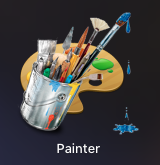
\includegraphics[scale=0.5]{dist.png}
    \caption{Painter程序}
\end{figure}


\section{开发环境}

\subsection{命令行版开发环境}

    \begin{quote}

        \begin{itemize}
            \item Python 3.7.7
            \item numpy 1.18.4
            \item Pillow 7.1.2
        \end{itemize}

    \end{quote}

\subsection{图形界面版开发环境}

    \begin{quote}

        \begin{itemize}
            \item Python 3.7.7
            \item PyQt5 5.14.2
            \item sip 5.2.0
            \item typing 3.7.4.1
        \end{itemize}

    \end{quote}    


注:以上是开发环境,因为开发中没有用到很偏门的特性,所以较低版本的库应该也可以运行。


\section{系统功能}


\subsection{界面总览}

\begin{figure}[H]
    \centering
    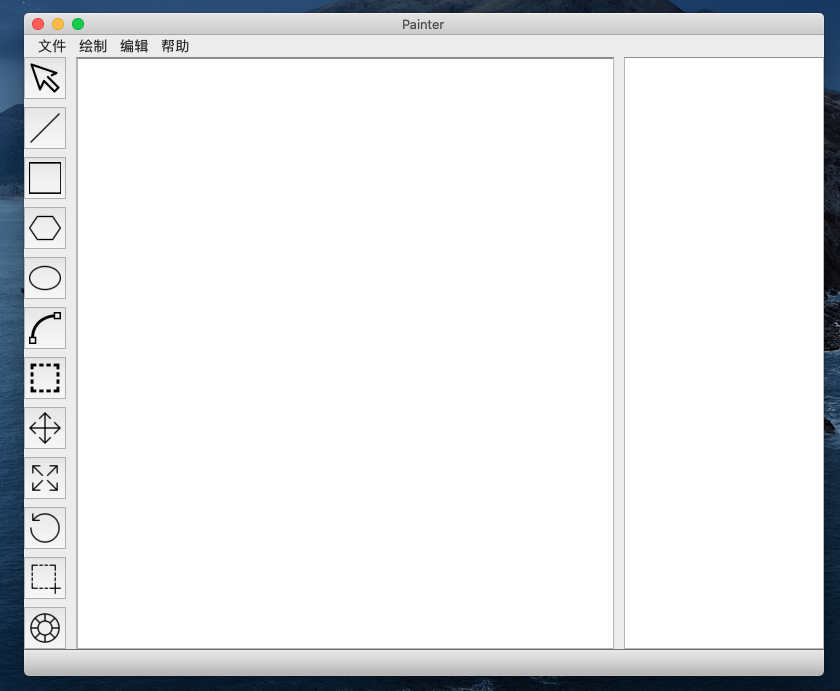
\includegraphics[scale=0.5]{Painter.png}
    \caption{Painter主界面}
\end{figure}

我们可以看到主界面可以一共分为四块:菜单栏,工具栏,画布,图元列表以及最下面的状态栏。


\subsubsection{菜单栏}

菜单栏中一共有四个子菜单:"文件", "绘制","编辑"和"帮助"。

"文件"子菜单主要是跟全局设置有关的,如设置画笔的颜色,重置画布,保存文件,退出等。

\begin{figure}[H]
    \centering
    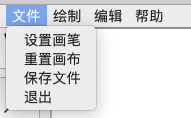
\includegraphics[scale=1.5]{menu_file.png}
    \caption{"文件"子菜单}
\end{figure}

"绘制"子菜单主要是用来绘制基本图元的,有的图元还可以选择具体的绘制算法。

\begin{figure}[H]
    \centering
    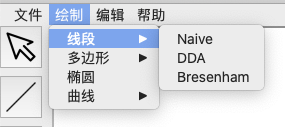
\includegraphics[scale=1.0]{menu_draw.png}
    \caption{"绘制"子菜单}
\end{figure}


"编辑"子菜单主要是用来对基本图形进行各种变换的,如平移,旋转,缩放和裁剪。其中裁剪操作可以指定算法。

\begin{figure}[H]
    \centering
    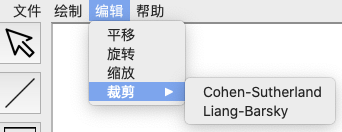
\includegraphics[scale=0.9]{menu_edit.png}
    \caption{"编辑"子菜单}
\end{figure}


"帮助"子菜单主要提供这个程序的一些信息。

\begin{figure}[H]
    \centering
    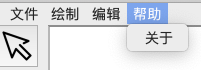
\includegraphics[scale=1.5]{menu_help.png}
    \caption{"关于"子菜单}
\end{figure}



\subsubsection{工具栏}

工具栏列出了一些常用的工具供用户使用,不必用户在菜单中选择,节省了用户的时间,也提高了易用性,而且每个工具上都有相应的简明图标的,而且当用户的鼠标移动到某一工具上时,还会自动提示该工具的功能。

\begin{figure}[H]
    \centering
    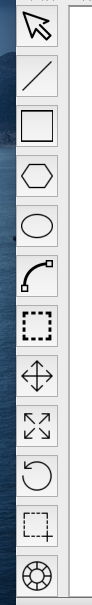
\includegraphics[scale=0.5]{toolbar.png}
    \caption{工具栏}
\end{figure}

\subsubsection{画布}

画布是用户主要的绘制区域,该画布的大小可以由用户任意指定,而且可以在有限的显示区域内通过鼠标任意滑动到用户想要的区域。

\subsubsection{图元列表}

\begin{figure}[H]
    \centering
    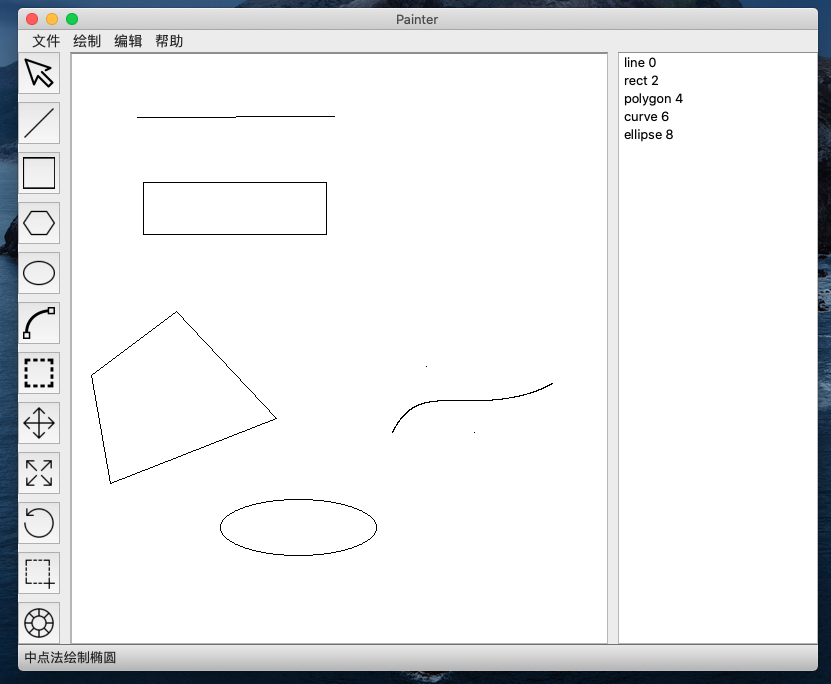
\includegraphics[scale=0.5]{item_list.png}
    \caption{图元列表}
\end{figure}

图元列表会列出所有用户已经绘制的图元,并通过友好的命名来标识。


\subsubsection{状态栏}

值得一提的是下面的状态栏,可以提示用户当前的状态,如上图中的就是"中点法绘制椭圆",在绘制的状态时会提醒用户当前用什么算法在绘制什么图元。

\subsection{绘制功能}

绘制直线:点击直线图标,默认的算法是DDA算法,你也可以在菜单栏里选择别的算法。然后在canvas区域按下鼠标左键标记直线的起点,然后不要松开鼠标,一直拖动到你想设定的终点,你松开的那个点就是直线的终点,在移动鼠标的过程你可以看到直线是在一直动态变化的。

绘制矩形:点击矩形图标,跟直线的画法类似,先按下鼠标的左键,然后拖动再松开。 我这里采用PyQt的矩形绘制,其实用户也可以通过多边形绘制矩形,这里是为了方便用户而增加的一个绘制矩形的功能,因为是PyQt的矩形所以不能通过我的旋转算法进行旋转,缩放和平移是没有问题的。

绘制多边形:点击多边形的图标,这里跟直线的画法就不太一样了,因为多边形可以有任意多个点,而直线只有两个点。所以用户每按一次鼠标的左键就会产生一个新的控制点,因为多边形是封闭的,所以用户每次最后按下的点会和第一个点进行连线,用户双击鼠标就表示多边形绘制完成。

绘制椭圆:点击椭圆图标,这里的画法和直线和矩形的画法是一样的,其实将相当于画出一个矩形,然后在里面画一个椭圆。

绘制曲线:点击曲线图标,默认的算法是Bezier算法,你可以在菜单栏里选择别的算法。然后跟绘制多边形一样,每次鼠标左键点击都会产生一个控制点,最后双击鼠标,就表示曲线绘制完成。

\subsection{图元变换功能}

要变换图元的话,你需要先用选择工具选择要变换的图元,被选中的图元会被红色的框所包围,就如下图所示。

\begin{figure}[H]
    \centering
    
\includegraphics[scale=0.5]{select.png}
    \caption{选择图元}
\end{figure}

平移图元:平移图元的操作就是拖动,按下鼠标然后拖动,鼠标的相对位移就对应着图元的相对位移。所有的图元都可以进行平移操作。

缩放图元:先选择一个缩放的中心点,然后鼠标从另外的任意一个点开始拖动,开始拖动的点和中心点有一个向量,拖动中的点和中心点也有一个向量,这两个向量在x方向上的倍数(可以为负数)就是缩放系数。所有的图元都可以进行缩放操作。

旋转图元:跟缩放图元类似,先选择一个缩放的中心点,然后鼠标从另外的任意一个点开始拖动,开始拖动的点和中心点有一个向量,拖动中的点和中心点也有一个向量。这两个向量的旋转角就是图元的旋转角度。除了椭圆和矩形其他的图元都可以进行旋转操作。


\subsection{其他功能}

重置画布:用户可以重置画布并指定画布的大小:

\begin{figure}[H]
    \centering
    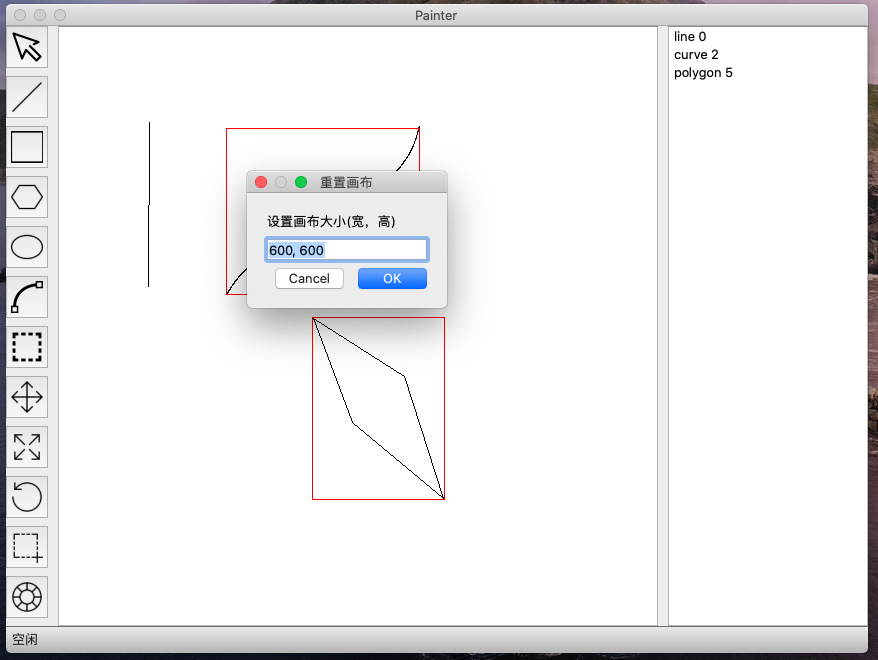
\includegraphics[scale=0.5]{reset.png}
    \caption{重置画布}
\end{figure}

设置画笔:用户可以通过调色板重新设置画笔的颜色,如下图,就设置了画笔为蓝色画了一个椭圆:

\begin{figure}[H]
    \centering
    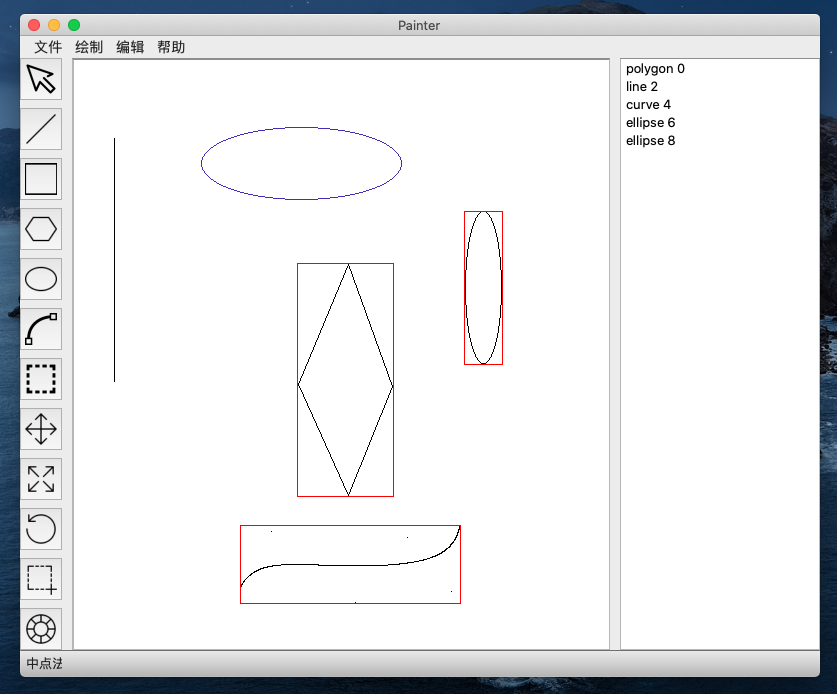
\includegraphics[scale=0.5]{color.png}
    \caption{设置画笔}
\end{figure}

保存文件:用户可以将自己的杰作保存成文件,支持png, jpg, bmp等格式,如下图我们就将刚刚的画作保存成了bmp文件:

\begin{figure}[H]
    \centering
    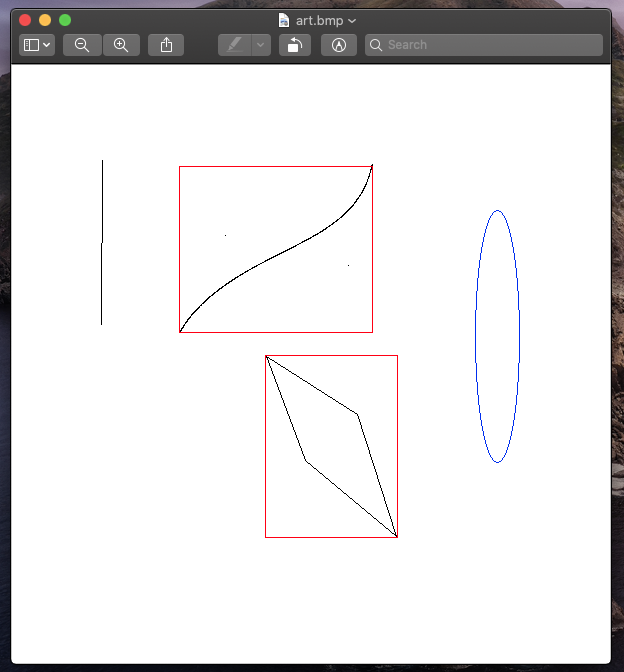
\includegraphics[scale=0.4]{save.png}
    \caption{保存文件}
\end{figure}
















%%%%%%%%%%%%%%%%%%%%

%%%%%%%%%%

%%%%%%%%%%

%%%%%%%%%%%%%%%%%%%%
\end{document}